\begin{frame}
	\frametitle{The SVN Model}
	\begin{block}{block}
		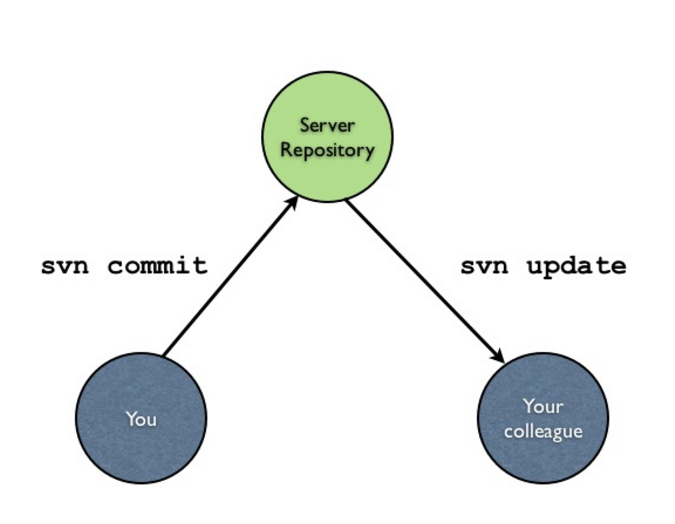
\includegraphics[width=\textwidth]{./images/svnmodel.png}
	\end{block}
\end{frame}
\begin{frame}
	\frametitle{The SVN Model}
	\begin{block}{block}
		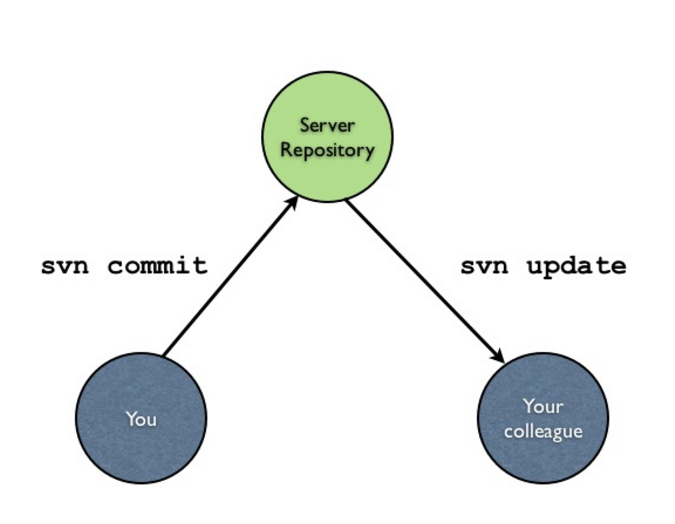
\includegraphics[width=\textwidth]{./images/svnmodel.png}
	\end{block}
\end{frame}
\begin{frame}
	\frametitle{Basic functionality}
	\begin{columns}
		\begin{column}{0.49\textwidth}
			\begin{block}{svn}
				\begin{itemize}
					\item checkout
					\item update
					\item commit
					\item log
					\item merge
					\item copy
					\item diff
					\item blame
				\end{itemize}
			\end{block}
		\end{column}
		\begin{column}{0.49\textwidth}
			\begin{block}{git}
				\begin{itemize}
					\item clone
					\item pull
					\item commit + push
					\item log
					\item merge/rebase
					\item branch/tag
					\item diff
					\item blame
				\end{itemize}
			\end{block}
		\end{column}
	\end{columns}
\end{frame}
